\chapter{Relativity}

An understanding of special relativity is necessary to properly understand much of particle physics.  Four vectors are defined by:

\[
  \begin{array}{ccccccc}
  x^{\mu} & = & (t,\ul{r}) & \quad & x_{\mu} & = & (t,-\ul{r}) \\
  p^{\mu} & = & (E,\ul{p}) & \quad & p_{\mu} & = & (E,-\ul{p}) 
  \end{array}
\]

Scalar products are given by:

\[
  \begin{array}{ccccccc}
  \ul{x}\cdot\ul{x} & = & x^{\mu}x_{\mu} & = & t^2 - x^2 &   & \\
  \ul{p}\cdot\ul{p} & = & p^{\mu}p_{\mu} & = & E^2 - p^2 & = & m^2
  \end{array}
\]

Also $x_{\mu} = g_{\mu\nu}x^{\nu}$, $x^{\nu} = g^{\nu\mu}x_{\mu}$.

where:

\begin{eqnarray*}
  g_{\mu\nu} & = &
  \left(
    \begin{array}{cccc}
    1 &  0 &  0 & 0 \\
    0 & -1 &  0 & 0 \\
    0 &  0 & -1 & 0 \\
    0 &  0 &  0 & -1
    \end{array}
  \right)
  \\
  g_{\mu\nu}g^{\mu\nu} & = & \displaystyle\sum_{\mu} \displaystyle\sum_{\nu} g_{\mu\nu}g^{\mu\nu} \\
  & = & \displaystyle\sum_{\mu}g_{\mu\mu}g^{\mu\mu} \\
  & = & \displaystyle\sum_{\mu}g_{\mu\mu}^2 \\
  & = & 4
\end{eqnarray*}

Recall that from quantum mechanics:

\[
  \begin{array}{ccc}
  E = i\frac{\partial}{\partial t} & \quad & \ul{p} = -i \ul{\nabla}
  \end{array}
\]

\begin{eqnarray*}
  \textrm{But } p^{\mu} = (E,\ul{p}) \\
  & = & i\left( \frac{\partial}{\partial t},-\ul{\nabla}\right) \\
  \textrm{So } p^{\mu} & = & i\partial^{\mu} \\
  \textrm{where } \partial^{\mu} & = & \left(\frac{\partial}{\partial t},-\ul{\nabla}\right) \\
  & = & \frac{\partial}{\partial x_{\mu}} \\
  \textrm{and } \partial_{\mu} & = & \left( \frac{\partial}{\partial t}, \ul{\nabla}\right) \\
  & = & \frac{\partial}{\partial x^{\mu}}
\end{eqnarray*}

Forming the De L'ambertian operator:

\[
  \partial^{\mu}\partial_{\mu} = \Box^2 = \left(\frac{\partial^2}{\partial t^2}, -\nabla^2\right)
\]

\section{Lorentz transformations}

A Lorentz transformation relates the coordinates in one frame to the coordinates of another frame.  By convention the lorentz transformation takes place along the (mutually parallel) $x$ axis, with velocity $v$.  $x'$ tranforms as:

\begin{eqnarray*}
  t'   & = & \gamma (t - vx_1)  \\
  x'_1 & = & \gamma (-vt + x_1) \\
  x'_2 & = & x_2 \\
  x'_3 & = & x_3 \\
  \gamma & = & \frac{1}{\sqrt{1-v^2}}
\end{eqnarray*}

The product $p^{\mu}q_{\mu}$ is invariant under a Lorentz transformation.

\section{The light cone}

Let $x^{\mu}$ denote the four vector $(x^0,\ul{x})$ and suppose light is emitted at $y^{\mu} = (y^0,\ul{y})$.  Consider the difference between $x^{\mu}$ and $y^{\mu}$:

\[
  s^2 = (x^{\mu} - y^{\mu})^2 = (x_0 - y_0)^2 - (\ul{x} - \ul{y})^2
\]

If the above is zero then:

\[
  (x^0 - y^0) = (\ul{x} - \ul{y})^2
\]

This is the equation of a light beam and defines a light cone.  If $s^2>0$ then the separation is time-like and the events are in the forward light cone and causally related.  If $s^2<0$ then the separation is space-like and the events have no causal connection.  The light cone is shown in figure \ref{fig:ch5_lightcone}.

\begin{figure}[!htb]
  \begin{center}
    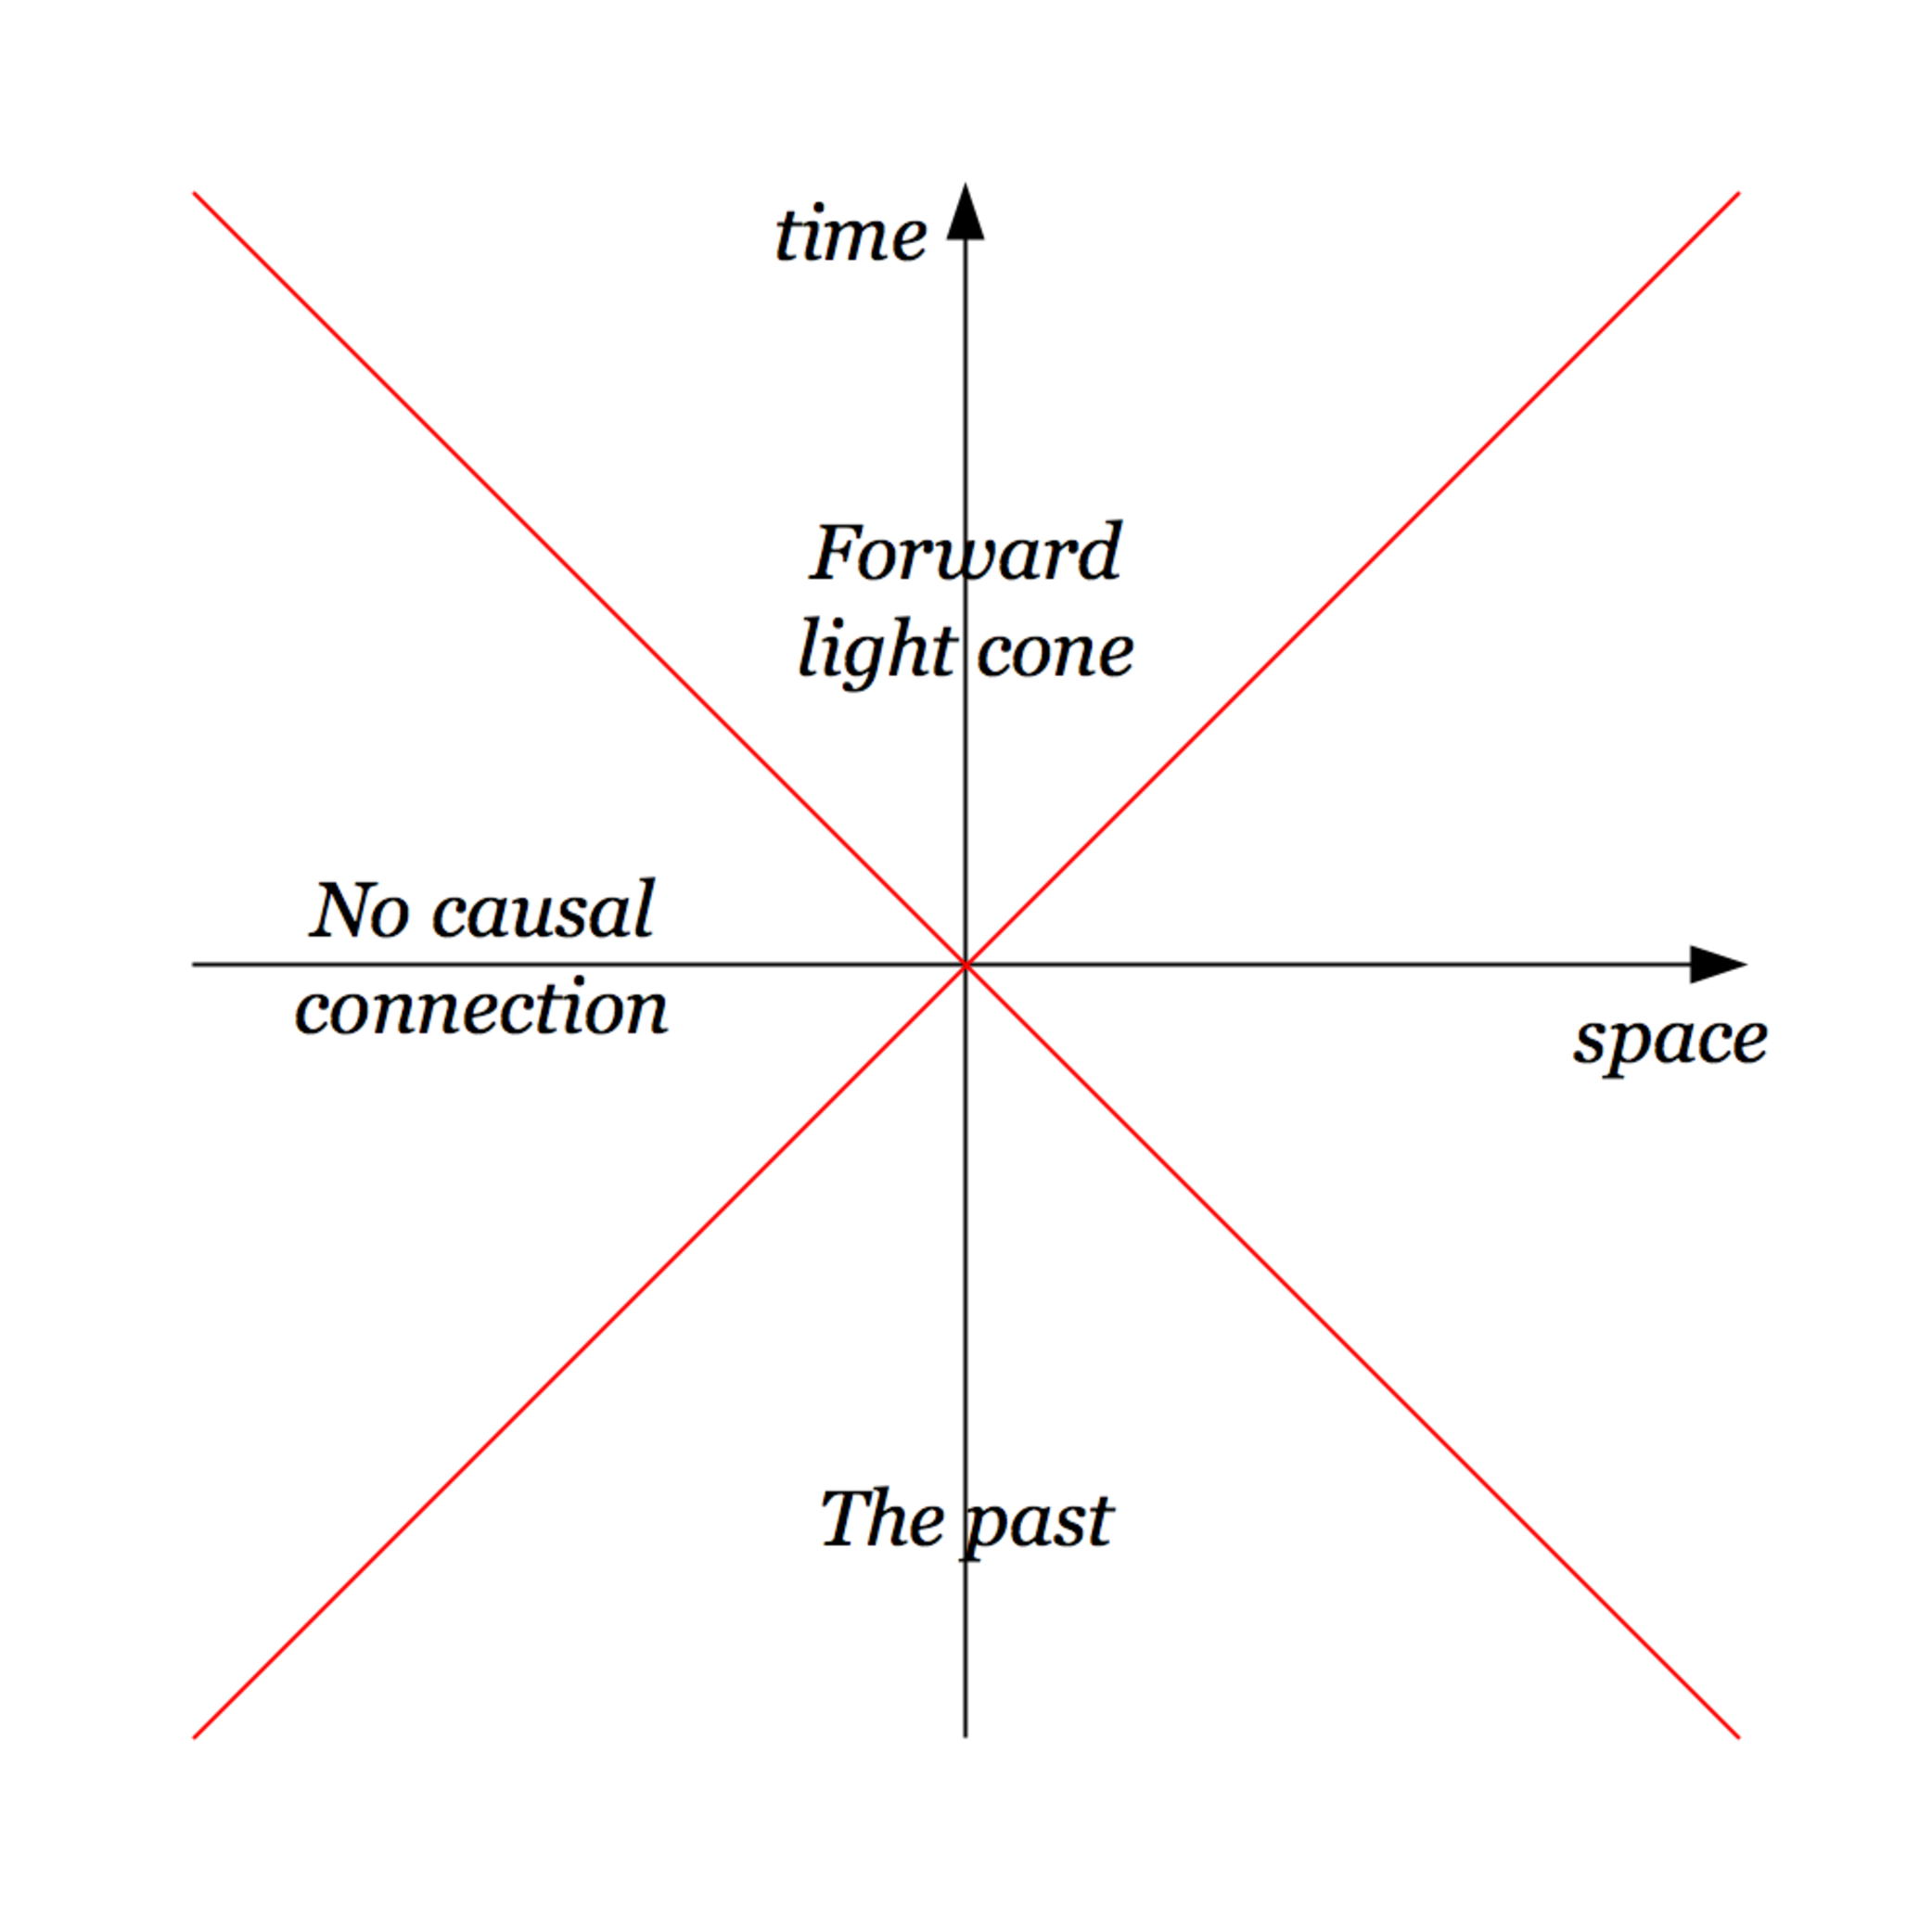
\includegraphics[width=0.75\textwidth]{images/chapter_5/lightcone.pdf}
    \caption[The light cone]{The light cone, showing distinct regions of spacetime which are and are not causally connected.  The red lines show the boundaries of these regions.}
    \label{fig:ch5_lightcone}
  \end{center}
\end{figure}

\section{Relativistic kinematics}

Usually, one of two processes is considered, either $A \to B + C$ (decay) or $A + B \to C + D$ (scattering).  For a decay the centre of mass energy is the mass of the particle $A$.  For scattering:

\[
  s = (p^{\mu}_A + p^{\mu}_B)^2 = (p^{\mu}_c + p^{\mu}_D)^2
\]

For a fixed target experiment $B$ is at rest:

\begin{eqnarray*}
  s & = & (E_A + E_B)^2 - (\ul{p}_A + \ul{p}_B)^2 \\
    & = & (E_A + m_B)^2 - P^2_A \\
    & = & m^2_A + m^2_B + 2m_BE_A \\
    \textrm{If } E_A & \gg & m_A, m_B \textrm{ then:} \\
    \sqrt{s} & \simeq & \sqrt{2E_A m_B}
\end{eqnarray*}

\subsection{Centre of mass frame}

\begin{eqnarray*}
  s & = & \left(p^{\mu}_A + p^{\mu}_B \right)^2 \\
    & = & \left(E^{CMS}_A + E^{CMS}_B\right)^2 - \left(p^{CMS}_A + p^{CMS}_B\right)^2 \\
    & = & \left(E^{CMS}_A\right)^2 + 2E^{CMS}_AE^{CMS}_B + \left(E^{CMS}_B\right)^2 \\
  \textrm{So } \sqrt{s} & = & E^{CMS}_A + E^{CMS}_B
\end{eqnarray*}

At Tevatron $E_P = E_{\bar{p}} = 980 GeV$, so $\sqrt{s} \simeq 2TeV$.

At HERA $E_p = 920GeV$, $E_e = 27.5GeV$, so $\sqrt{s} = 318GeV$.

To transform between the centre of mass frame and the laboratory frame it is necessary to determine $\beta$ and $\gamma$:

\begin{eqnarray*}
  \beta & = & \frac{\textrm{Three momentum part of four vector}}{\textrm{Energy part of four momentum}} \\
  & = & \frac{|\ul{p}_A| + |\ul{p}_B|}{E_A + E_B} \\
  \gamma & = & \frac{\textrm{Energy part of four momentum}}{\textrm{Centre of mass energy}} \\
  & = & \frac{|\ul{p}_A| + |\ul{p}_B|}{\sqrt{s}}
\end{eqnarray*}

The energy and momentum of a particle in the centre of mass frame can be determined using invariance rather than Lorentz transformations:

\begin{eqnarray*}
  p^{\mu}_A + p^{\mu}_B & = & \left(\sqrt{s},0\right) \textrm{ in the centre of mass frame} \\
  p_{A\mu}\left(p^{\mu}_A + p^{\mu}_B \right) & = & \left(E^{CMS}_A,\ul{p}^{CMS}_A\right) \cdot \left(\sqrt{s},0\right) \\
  \Rightarrow p_{A\mu} \left(p^{\mu}_A + p^{\mu}_B\right) & = & E^{CMS}_A \sqrt{s} \\
  m^2_a + p_{A\mu}p^{\mu}_B & = & E^{CMS}_A \sqrt{s} \\
  \textrm{Recall } s & = & \left( p^{\mu}_A + p^{\mu}_B\right)\left(p_{A\mu} + p_{B\mu}\right) \\
  & = & p_A \cdot p_A + p_B \cdot p_B + 2p^{\mu}_A\cdot p_{B\mu} \\
  \textrm{So } p_{A\mu}p^{\mu}_B & = & \frac{s - m^2_A - m^2_B}{2} \\
  \textrm{So } E^{CMS}_A & = & \frac{2m^2_A + s - m^2_A - m^2_B}{2\sqrt{s}} \\
  \Rightarrow E^{CMS}_A & = & \frac{s + m^2_A - m^2_B}{2\sqrt{s}}
\end{eqnarray*}

And similarly for the other energies.

\begin{eqnarray*}
  \left( p^{CMS}_A \right)^2 & = & \left( E^{CMS}_A \right)^2 - m^2_A \\
  \textrm{So } \left(p^{CMS}_A\right)^2 & = & \left( \frac{s + m^2_A - m^2_B}{2\sqrt{s}}\right)^2 - m^2_A \\
  & = & \frac{\left(s + m^2_A - m^2_B\right)^2}{4s}-m^2_A \\
  & = & \frac{s^2 + \left(m^2_A - m^2_B\right)^2 + 2sm^2_A - 2sm^2_B - 4sm^2_A}{4s} \\
  & = & \frac{s^2 + \left(m^2_A - m^2_B\right)^2 - 2s\left(m^2_A + m^2_B\right)}{4s} \\
  & = & \frac{\lbrack s - \left(m_A + m_B\right)^2\rbrack \lbrack s - \left(m_A - m_B\right)^2 \rbrack}{4s}
\end{eqnarray*}

\subsection{Mandelstan variables}

The Mandelstan variables are shown in figure \ref{fig:ch5_mandelstan}.

\begin{figure}[!htb]
  \begin{center}
    \begin{tabular}{ccc}
      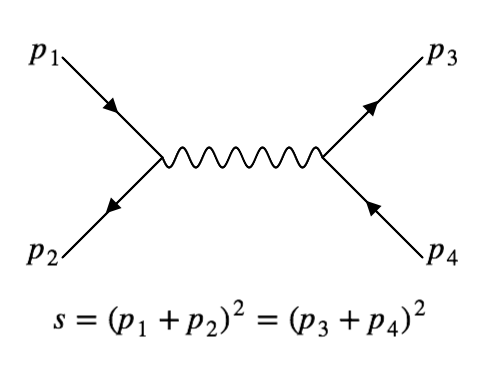
\includegraphics[width=0.4\textwidth]{images/web_feynman/image_17.png}
      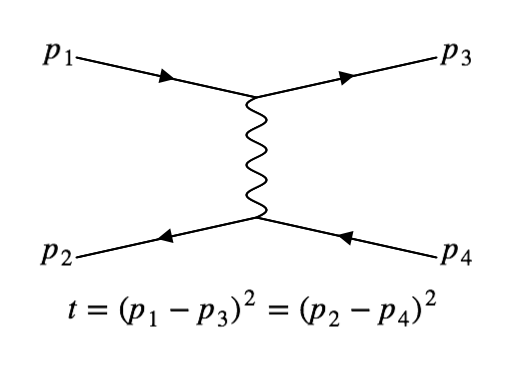
\includegraphics[width=0.4\textwidth]{images/web_feynman/image_18.png}
      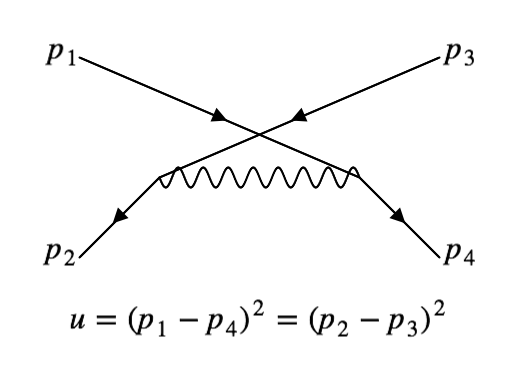
\includegraphics[width=0.4\textwidth]{images/web_feynman/image_19.png}
    \end{tabular}
    \caption[Mandelstan variables]{The Mandelstan variables are relativistically invariant kinematic quantities.}
    \label{fig:ch5_mandelstan}
  \end{center}
\end{figure}

\begin{eqnarray*}
  s & = & \left(p_A + p_B\right)^2 \\
  t & = & \left(p_A - p_C\right)^2 \\
    & = & \left(p_B - p_D\right)^2 \\
    & = & -Q^2 = q^2 \\
  u & = & \left(p_A - p_D\right)^2 \\
    & = & \left(p_C - p_B\right)^2 \\
    s + t + u & = & m^2_A + m^2_B + m^2_C + m^2_D \\
    \textrm{Proof: } s + t + u & = & \left(p_A + p_B\right)^2 + \left(p_A - p_C\right)^2 + \left(p_A - p_D\right)^2 \\
    & = & p^2_A + P^2_B + 2p_Bp_A + p^2_A + p^2_C - 2p_Ap_C + p^2_A + p^2_D - 2p_Ap_D \\
    & = & 3m^2_A + m^2_B + m^2_C + m^2_D + 2\left(p_Bp_A - p_Ap_C - p_Ap_B\right) \\
    & = & 3m^2_A + m^2_B + m^2_C + m^2_D + 2p_A\left(p_B - p_C - p_D\right) \\
    \textrm{But } p_A + p_B & = & p_C + p_D \\
    \Rightarrow p_B - p_C - p_D & = & -p_A \\
    \textrm{So } s + t + u & = & m^2_A + m^2_B + m^2_C + m^2_D
\end{eqnarray*}

\section{Relativistic spin\texorpdfstring{$-0$}{-0} particles}

\subsection{The Klein-Gordon equation}

The quantum wavefunction for a free scalar particle propagating in the $x-$direction is:

\begin{eqnarray*}
  \phi & \sim & \e^{i(px - Et)} \\
       & \sim & \e^{ip^{\mu}x_{\mu}}
\end{eqnarray*}

Repeating the procedure that yielded the Schroedinger equation, but using:

\begin{equation}
  E^2 = p^2 + m^2 \textrm{ (rather than }E = p^2/2m\textrm{)} \label{eq:relativisticmass}
\end{equation}

\begin{equation}
  \begin{array}{ccc}
  E & \to & i\frac{\partial}{\partial t} \\
  \ul{p} & \to & -i\ul{\nabla}
  \end{array}
  \Bigg\}
  \label{eq:relativisticep}
\end{equation}

Combining (\ref{eq:relativisticmass}) and (\ref{eq:relativisticep}) and transforming in an equation acting on $\phi$ gives:

\begin{eqnarray}
  \frac{\partial^2\phi}{\partial t^2} & = & -\nabla^2\phi + m^2\phi
  \label{eq:kleingordon} \\
  \textrm{Or } \Box^2\phi & = & m^2 \phi \nonumber
\end{eqnarray}

(\ref{eq:kleingordon}) is the Klein-Gordon equation (or the relativistic Schroedinger equation.  The complex conjugate of (\ref{eq:kleingordon}) is:

\begin{eqnarray}
  -\frac{\partial^2\phi^{\star}}{\partial t^2} = & -\nabla^2\phi^{\star} + m^2\phi^{\star} &\label{eq:kleingordonconjugate} \\
  \phi^{\star}\times(\ref{eq:kleingordon}) = & -\phi^{\star}\frac{\partial^2\phi}{\partial t^2} & = -\phi^{\star}\nabla^2\phi + m^2\phi^{\star}\phi \label{eq:phistarphi} \\
  \phi\times(\ref{eq:kleingordonconjugate}) = & -\phi\frac{\partial^2 \phi^{\star}}{\partial t^2} & = -\phi\nabla^2\phi^{\star} + m^2\phi\phi^{\star} \label{eq:phiphistar} \\
  -i\left( (\ref{eq:phistarphi}) - (\ref{eq:phiphistar}) \right) = & i\left( \phi^{\star}\frac{\partial^2\phi}{\partial t^2}- \phi\frac{\partial^2\phi}{\partial t^2}\right) & = i\left(\phi^{\star}\nabla^2\phi - \phi\nabla^2\phi^{\star} \right) \nonumber
\end{eqnarray}
\begin{eqnarray}
  \Rightarrow i \frac{\partial}{\partial t}\Bigg[ \phi^{\star}\frac{\partial \phi}{\partial t} - \phi\frac{\partial \phi^{\star}}{\partial t}\Bigg] - i\ul{\nabla}\lbrack \phi^{\star}\ul{\nabla}\phi - \phi\ul{\nabla}\phi_{\star}\rbrack & = 0 & \nonumber \\
  \textrm{or } \frac{\partial \rho}{\partial t} + \ul{\nabla}\cdot\ul{j} & = 0 & \nonumber
\end{eqnarray}

\begin{eqnarray*}
  \rho & = & i\left(\phi^{\star}\frac{\partial\phi}{\partial t} - \phi\frac{\partial \phi^{\star}}{\partial t} \right) \\
  \ul{J} & = & i\left( \phi^{\star}\ul{\nabla}\phi - \phi\ul{\nabla}\phi^{\star}\right) 
\end{eqnarray*}

Consider the form of $\rho$ for $\phi = N\e^{i\ul{p}\cdot{\ul{x}}}$:

\begin{eqnarray*}
  \phi & = & N\e^{i\left(px - Et\right)} \\
  \rho & = & i\left(\phi^{\star}\frac{\partial \phi}{\partial t} - \phi \frac{\partial \phi^{\star}}{\partial t}\right) \\
  & = & i \left( N^{\star}\e^{-i\left(px-Et\right)}\left(-iE\right)N\e^{i\left(px-Et\right)} - N\e^{i\left(px-Et\right)}\left(iE\right)N^{\star}\e^{-1\left(px-Et\right)}\right) \\
  & = & i\lbrack N^{\star}N\left(-iE\right) - NN^{\star}\left(ie\right) \rbrack \\
  & = & 2N^{\star}NE \\
  \textrm{So } \rho & = & 2EN^{\star}N
\end{eqnarray*}

Similarly $\ul{j} = 2N^{\star}N\ul{p}$.

This appeared disastrous because $E^2 = p^2 + m^2$ lead to negative energy solutions (ie $E_- = -\sqrt{p^2 + m^2}$) which lead to negative probability densities, $\rho<0$.  Note that $\rho$, being proportional to $E$ may have been antiticipated.  Under a Lorentz boost of speed $v$ the volume element undergoes a contraction:

\[
  \mathrm{d}^3r \to \gamma\mathrm{d}^3r
\]

Therefore to keep $\rho \mathrm{d}^3r$ invariant $\rho$ must transform as a time-like component:
\[
  \rho \to \gamma \rho
\]

\subsection{The perceived distaster of the Klein-Gordon equation}

The problem faced is that the Klein-Gordon equation can give $\rho<0$.  There are two steps to remove this problem which works for scalar particles.  In 1934 Pauli and Weisskopf derived the Klein-Gordon equation by multiplying $\ul{j} = \left(\rho, \ul{j}\right)$ by the charge of the particle, so $q\ul{j}^{\mu}$ becomes $\ul{j}^{\mu}_{em}$:

\[
  \ul{j}^{\mu}_{em} = -i\e\left(\phi^{\star}\partial^{\mu}\phi - \phi\partial^{\mu}\phi^{\star} \right)
\]

where $-\e$ is the charge on the scalar electron.  Now $\rho = j^0_{em}$ is a charge densiity and not a probability density, so $\rho$ can be negative.

\subsection{The Feynmann-Stueckelberg interpretation of \texorpdfstring{$E<0$}{ELO0} solutions}

The approach taken by Feynmann and Stueckelberg is that the negative energy solutions describe a negative energy particle propagating backwards in time or equivalently, a positive energy antiparticle propagating forwards in time.  Consider an electron of energy $E$, momentum $\ul{p}$ and charge $-\e$:

\[
  \ul{j}_{em}(\e^-) = -2eN^{\star}N(E,\ul{p})
\]

For a positron the charge is $\e$:

\[
  \ul{j}_{em}(\e^+) = 2\e N^{\star}N(E,\ul{p})
\]

which is equivalent to:

\[
  \ul{j}_{em}(\e^-) = -2\e N^{\star}N(-E,-\ul{p})
\]

which is the same as $\ul{j}_{em}$ but with $(-E,-\ul{p})$ so the emission of a positron of energy $E$ is the same as the absorption of an electron with energy $-E$.  These ideas can describe many particle interactions.  Consider a double scattering process in an interaction region, as shown in figure \ref{fig:ch5_paths}.

\begin{figure}[!htb]
  \begin{center}
    \begin{tabular}{cc}
      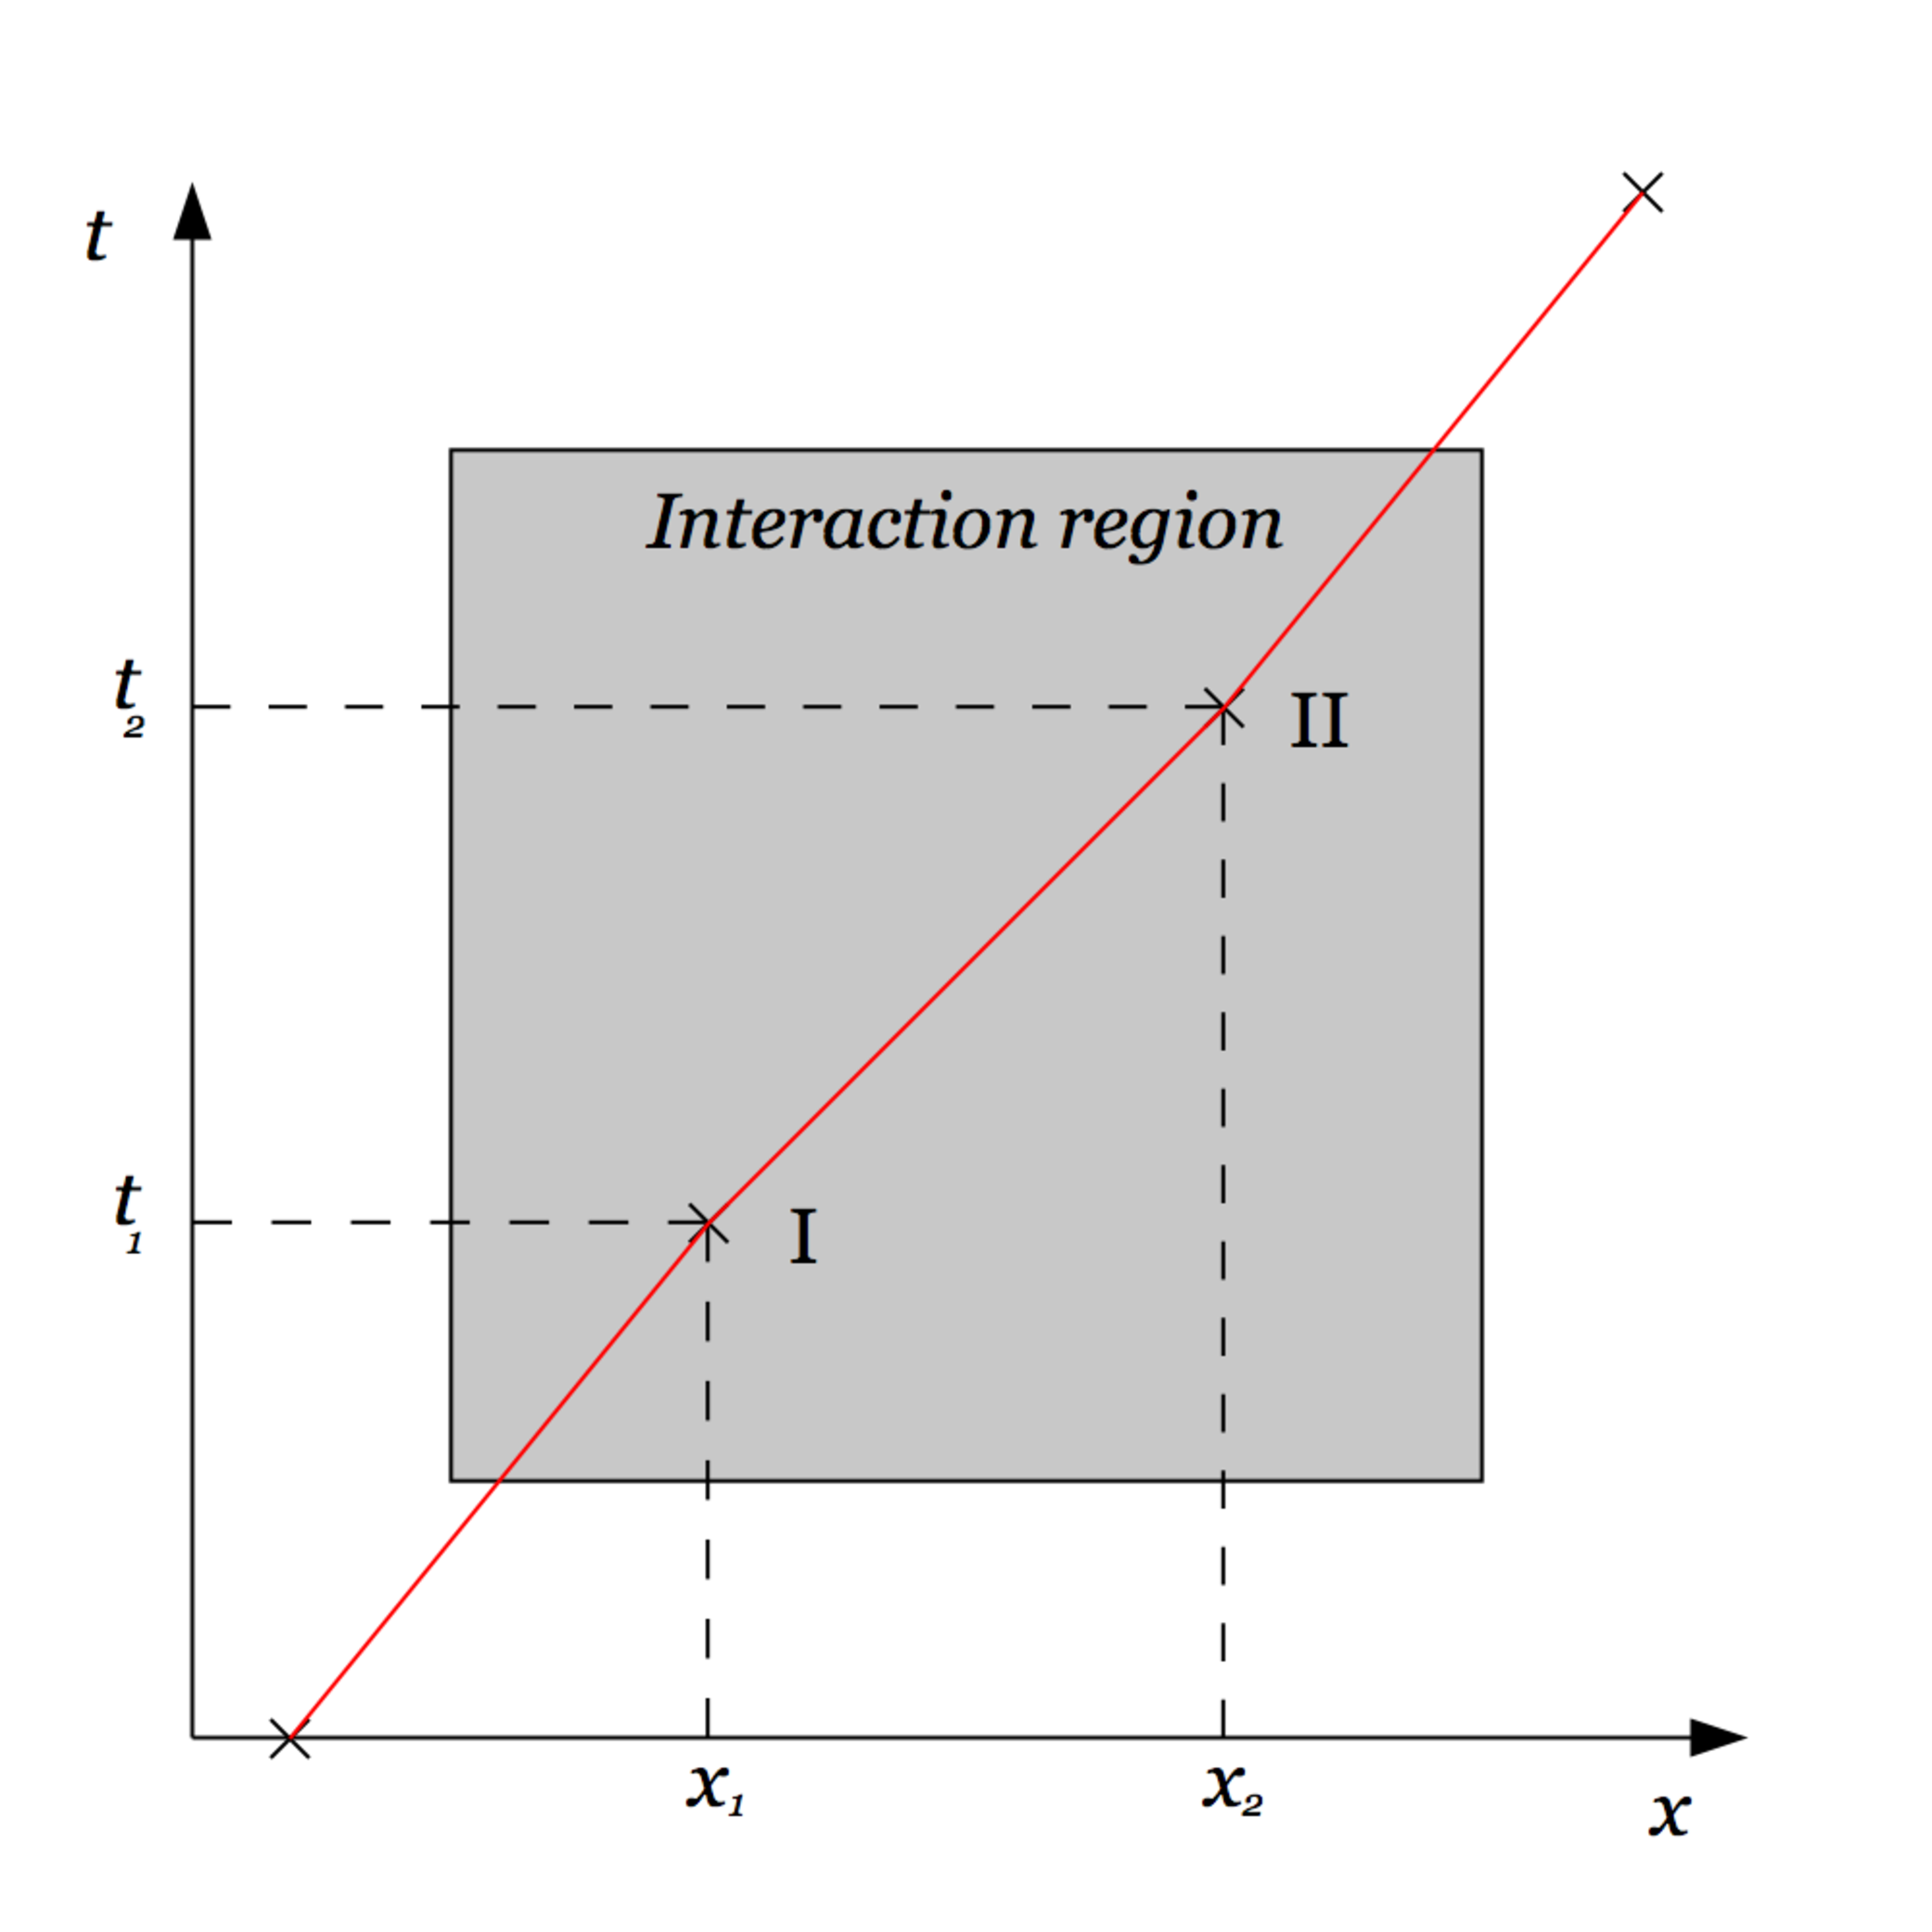
\includegraphics[width=0.5\textwidth]{images/chapter_5/path1.pdf} &
      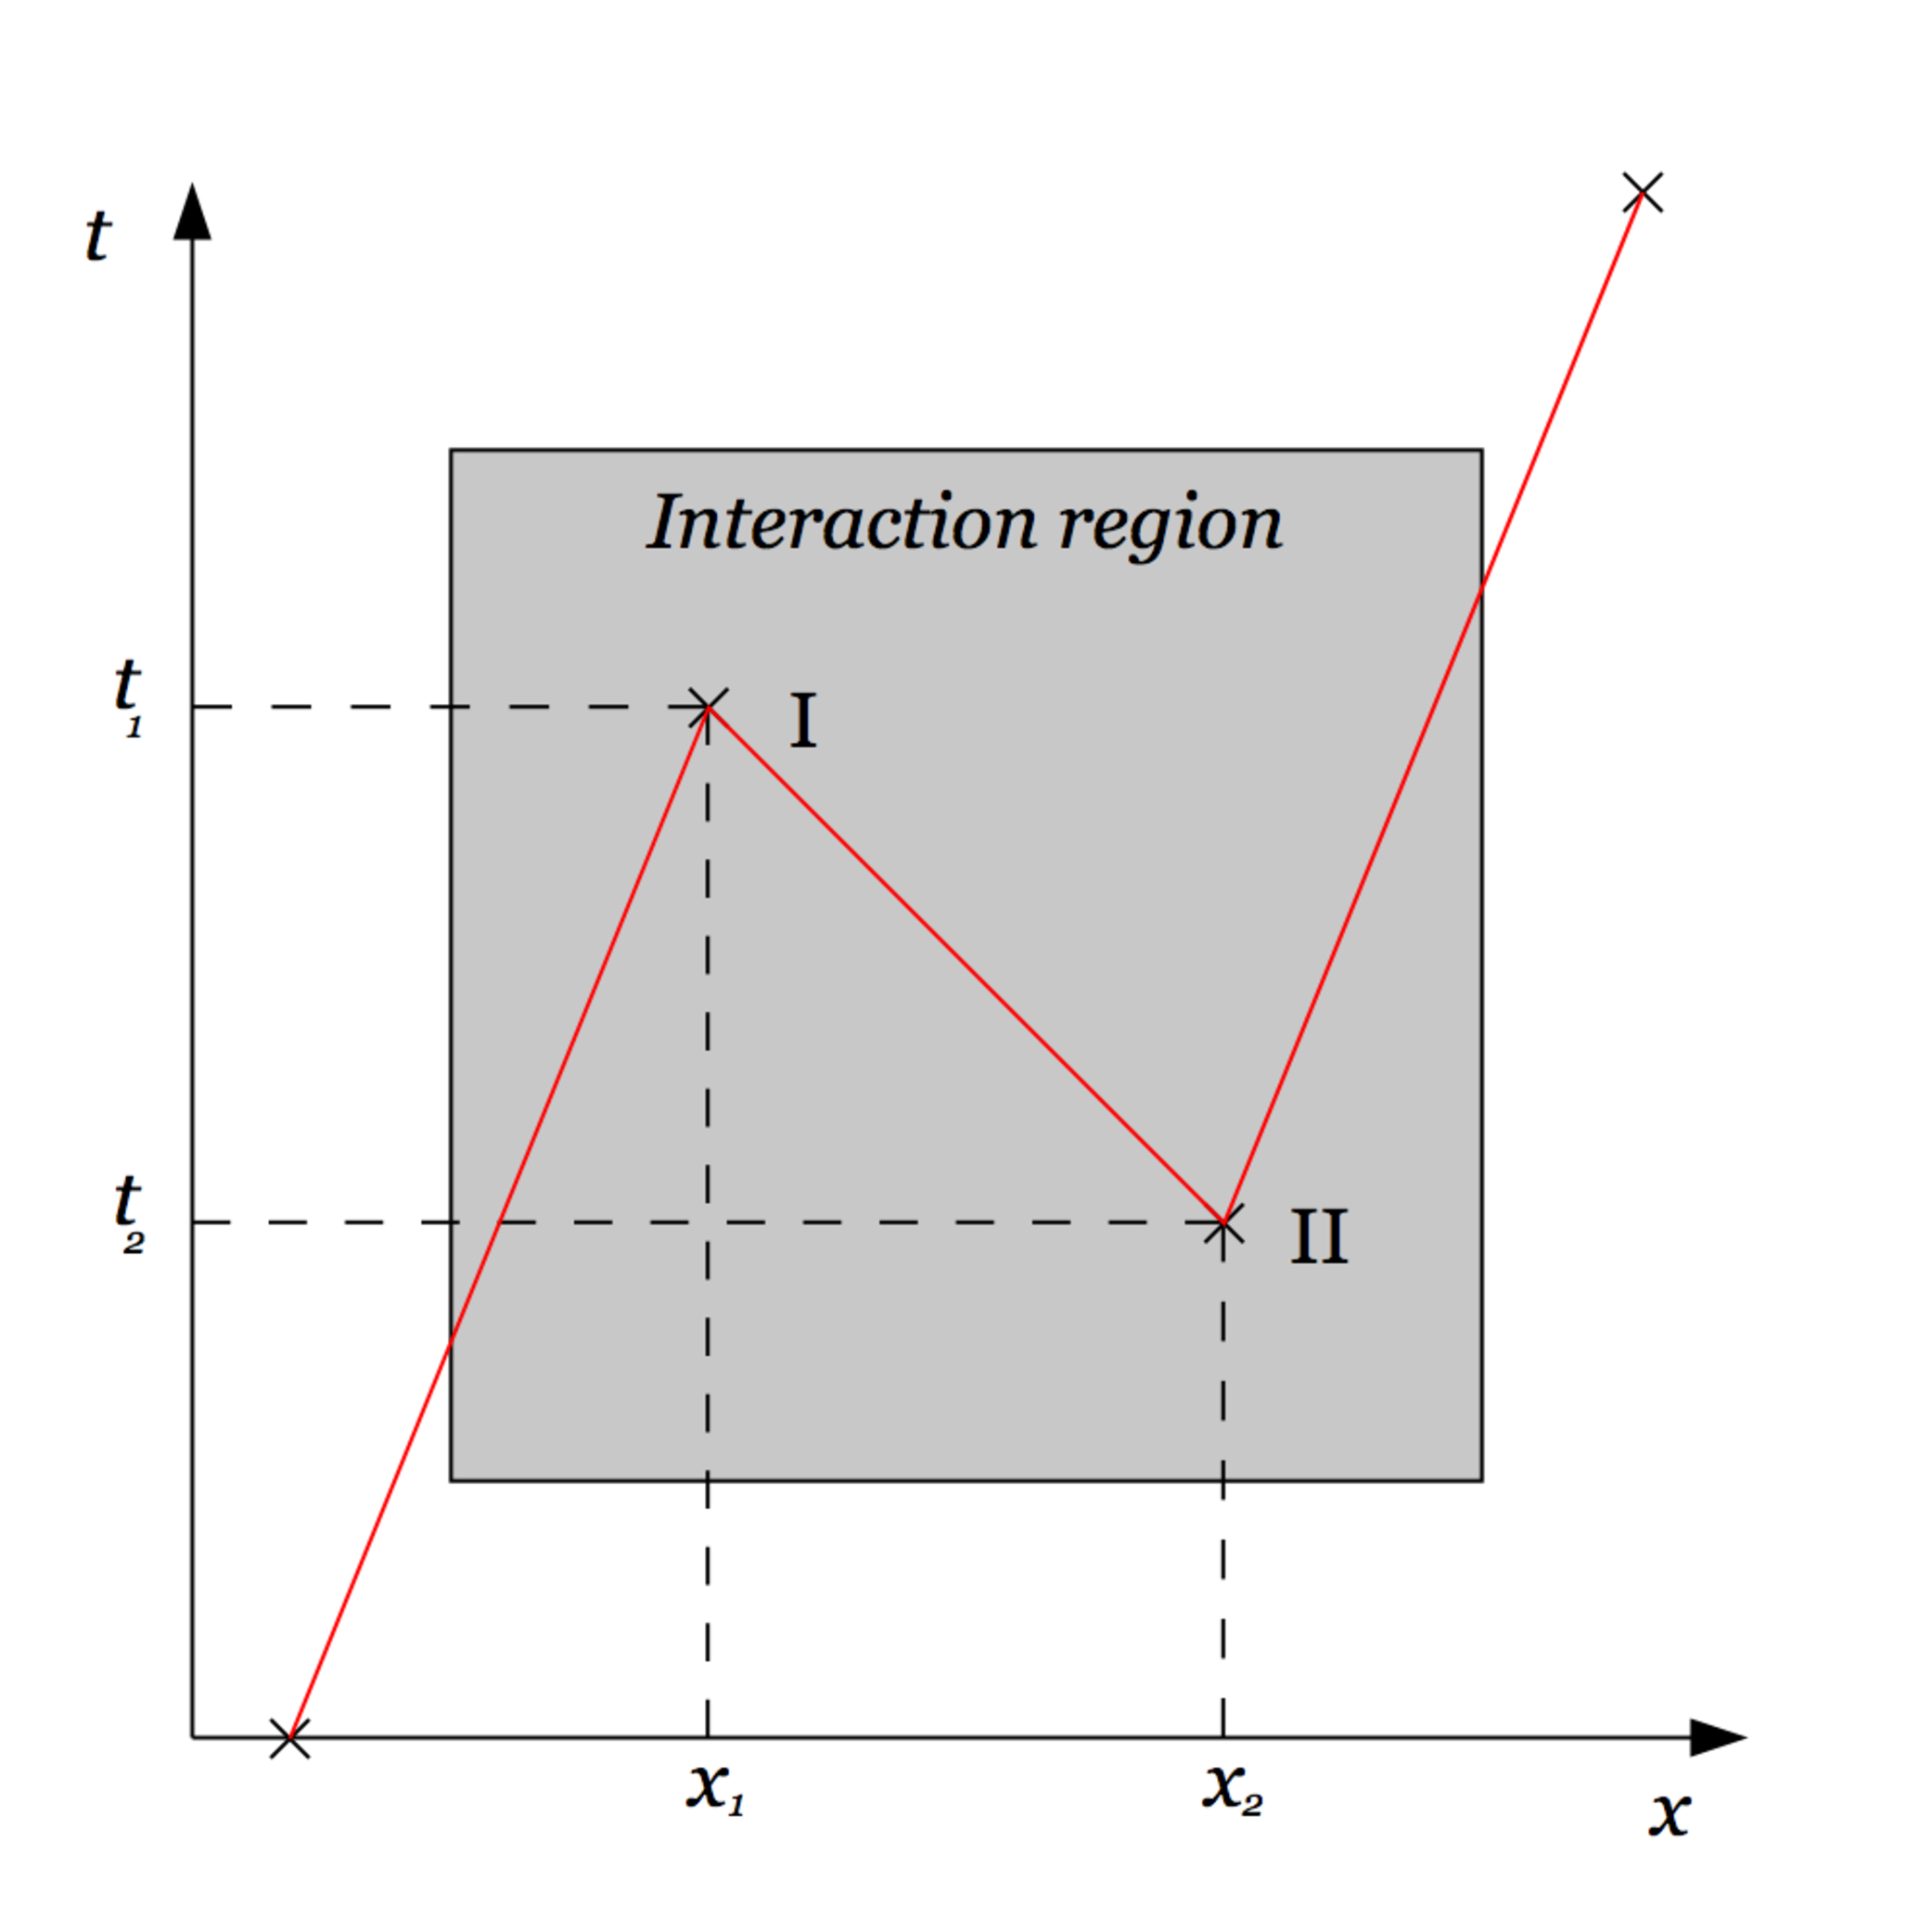
\includegraphics[width=0.5\textwidth]{images/chapter_5/path2.pdf} \\
    \end{tabular}
    \caption[A causal and a non-causal path of a particle]{Two paths of a particle, one of which respects causality (left), and one of which violates causality (right).}
    \label{fig:ch5_paths}
  \end{center}
\end{figure}

For the first diagram, at time $t_1$ and position $\ul{r}_1$ the electron scatters at $I$ and then at a later time $t_2$ and position $\ul{r}_2$ scatters at $II$.  All particles go forwards in time.  For the second diagram, at the earlier time $t_1$ and position $\ul{r}_1$ an electron-positron pair is created at $I$.  The electron leaves the volume and the positron propagates forwards in time to $t_2$ and $\ul{r}_1$ where it annihilates with an electron at $II$.

Both of the above diagrams have the same initial and final state, but the first involves just one electron while the second involves three particles.  They would both have to be included when calculating the probability of that process occuring.
